\documentclass[12pt,a4paper,utf8x]{report}
\usepackage [frenchb]{babel}

\usepackage{graphicx}
\usepackage{caption}
\usepackage[utf8x]{inputenc}
\usepackage{multicol}
\usepackage{url} % Pour avoir de belles url
\usepackage {geometry}
\usepackage {listings} %Pour mettre du code source 
\usepackage{verbatim}
%\usepackage{lscape} % Pour pouvoir passer en paysage
\usepackage{colortbl}
\usepackage{xcolor}
\usepackage{textcomp}
\usepackage[strings]{underscore}

\geometry{left=2.5cm,right=2.5cm,vmargin=2cm}
\usepackage[pdftex,bookmarks = true,bookmarksnumbered = true,pdfpagemode = None,pdfstartview = FitH,pdfpagelayout = OneColumn,colorlinks=true,linkcolor=black,urlcolor=blue,citecolor=blue,pdfborder = {0 0 0}]{hyperref}


%chapitre---------------------------------------------------------------------
 
%%%% debut macro pour enlever le nom chapitre %%%%
\makeatletter
\def\@makechapterhead#1{%
  \vspace*{50\p@}%
  {\parindent \z@ \raggedright \normalfont
    \interlinepenalty\@M
    \ifnum \c@secnumdepth >\m@ne
        \Huge\bfseries \thechapter\quad
    \fi
    \Huge \bfseries #1\par\nobreak
    \vskip 40\p@
  }}

\def\@makeschapterhead#1{%
  \vspace*{50\p@}%
  {\parindent \z@ \raggedright
    \normalfont
    \interlinepenalty\@M
    \Huge \bfseries  #1\par\nobreak
    \vskip 40\p@
  }}
\makeatother
%%%% fin macro %%%% 

\begin{document}

\begin{titlepage}
\begin{flushright}
   	
\includegraphics[scale=0.30]{univorleans.png}\\ 
   	   	Département Informatique
\end{flushright}
\vspace{30mm}
\begin{center}
\huge{Rapport de projet réseau}\\
\vspace{8mm}
\vspace{3mm}
\large{Proposé par : Sophie Robert}
\vspace{3mm}
\large{\\Réalisé par :}\\
\large{Fontorbe Jordan, Guillaume Arthur}\\
\end{center}
\begin{figure}[b!]
\begin{flushright}
~~\\ ~~\\ ~~\\ ~~\\ ~~\\ ~~\\ ~~\\
\large{Année universitaire: 2012-2013}
\end{flushright}
\end{figure}
\end{titlepage}

\tableofcontents
\clearpage

\chapter[Architecture des réseaux]{Présentation de l'architecture des réseaux}
Pour réaliser ce projet, nous disposions d'un réseau Netkit fournit avec le sujet.\\
Celui-ci se compose de plusieurs sous-réseaux:
\begin{description}
\item[hub]Le sous-réseau que nous avons dû configurer. Il est composé d'un routeur \emph{box} et de deux machines \emph{pc1} et \emph{pc2}. La configuration de ce sous-réseau que nous avons dû effectuer devait être faite uniquement à travers le routeur \emph{box}.
\item[rezo]Un sous-réseau extérieur à \emph{hub}. Celui-ci devait pouvoir communiquer avec \emph{hub}. Il n'était pas autorisé de modifier la configuration des machines de ce sous-réseau. Ce sous-réseau contient deux machines dont un serveur web.
\end{description}
\begin{center}
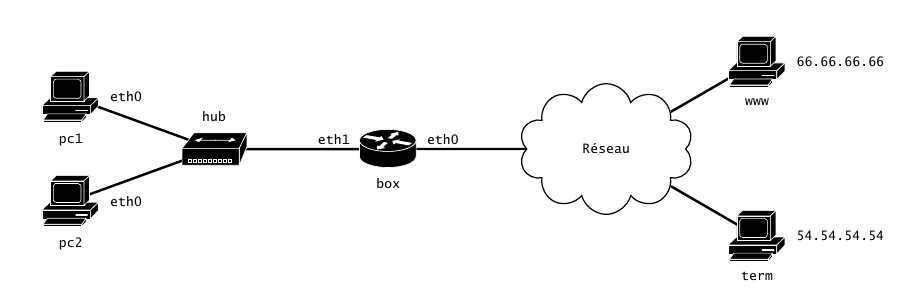
\includegraphics[scale=0.5]{archi.png}
\end{center}
\chapter{Travail effectué}
\section{Configuration du routeur}
Cette première partie consistait en la configuration du routeur \emph{box} pour que celui-ci puisse communiquer avec les réseaux extérieurs et avec les machines du sous-réseau \emph{hub}.\\
Pour cela nous avons éditer le fichier \emph{box.startup} comme suit:
\begin{verbatim}
ifconfig eth0 110.186.156.14
ifconfig eth1 10.176.63.1
route add default gw 110.0.0.1
\end{verbatim}
Les deux premières lignes servent à configurer statiquement les adresses IP des deux interfaces du routeur \emph{box}.\\
L'interface \textbf{eth1} est dans le sous-réseau \emph{hub} alors que \textbf{eth0} permet de communiquer avec le reste du monde.\\
La troisième ligne indique au routeur la passerelle par défaut qui permettra de communiquer avec les machines qui ne sont les sous-réseaux auxquels il appartient.
\section{Configuration du serveur DHCP}
Cette deuxième partie, a pour but de configurer un serveur DHCP sur le routeur \emph{box} afin d'attribuer des adresses IP de façon dynamique aux machines du réseau.
\begin{verbatim}
default-lease-time 3600;
max-lease-time 86400;

subnet 10.176.63.0 netmask 255.255.255.224{
       range 10.176.63.3 10.176.63.30;
       option routers    10.176.63.1;
}
\end{verbatim}
Les deux premières lignes permettent de configurer les durées de validité des baux accordés par le serveur.
La valeur 3600 a été choisit arbitrairement. Elle est exprimée en secondes. Une durée de validité courte est privilégiée pour des sous-réseaux avec beaucoup de machines afin de pouvoir réutiliser les adresses rapidement après la déconnexion d'un client. A contrario une durée de validité plus longue sera privilégié pour réduire le trafic dans le sous-réseau.\\
Les trois lignes suivantes servent à attribuer dynamiquement une adresse IP comprise entre 10.176.63.3 et 10.176.63.30 sur le réseau privé 110.176.63.0/27 aux clients souhaitant rejoindre le réseau.
L'adresse 10.176.63.0 est celle du réseau et ne peut donc pas être attribuée à une machine. Tout comme 10.176.63.31 qui est l'adresse de broadcast de ce sous-réseau.\\
Enfin, l'adresse 10.176.63.2 est réservé pour une machine particulière du sous-réseau. Ceci sera détaillé dans le point 4 de ce chapitre (l'adresse 10.176.63.1 est utilisée par le routeur \emph{box}).
La dernière ligne sert à indiquer la passerelle par défaut aux machines se configurant via le serveur DHCP. 
\end{document} 
